\input{header.tex}
\input{newcommands.tex}


\title{Multiple-Choice-Fragen mit \hologo{LaTeX} erstellen}
\author{Fortbildungsmaterial für MINT-Lehrkräfte}
\date{13. Mai 2025}
\pagestyle{plain}

\begin{document}

\maketitle

Multiple-Choice-Fragen (MC-Fragen) sind ein weit verbreitetes Format in Prüfungen, Tests und Arbeitsblättern. Mit \hologo{LaTeX} lassen sich solche Fragen systematisch und einheitlich gestalten. Durch die Definition eigener Befehle und Umgebungen wird die Erstellung von MC-Fragen erheblich vereinfacht und konsistenter. Diese Handreichung zeigt, wie Sie eigene Befehle und Umgebungen für verschiedene Arten von MC-Fragen definieren und anwenden können.



%%%%  KAPITEL 1  %%%%
\section{Grundlagen zum Erstellen eigener Befehle und Umgebungen}

Bevor wir in die spezifische Implementierung von MC-Fragen einsteigen, wiederholen wir kurz die grundlegenden Konzepte von \texttt{\textbackslash newcommand} und \texttt{\textbackslash newenvironment}.

\subsection{Einfache Befehlsdefinition mit \texttt{\textbackslash newcommand}}

Mit \texttt{\textbackslash newcommand} können wir eigene Befehle definieren:

\begin{lstlisting}[style=latex]
% Syntax: \newcommand{\befehlsname}[anzahl_parameter][standardwert]{definition}
\newcommand{\casket}{\LARGE{$\square$}}
\end{lstlisting}

Im vorliegenden Beispiel wird unser Antwortkästchen definiert.  Das Kommando \texttt{\textbackslash LARGE} vergrößert das mathematische Symbol \texttt{\textbackslash square}, das aus dem \texttt{amssymb}-Paket stammt. Dieser neue Befehl \texttt{\textbackslash casket} erzeugt nun ein großes leeres Quadrat – perfekt für die Ankreuzkästchen in unseren MC-Fragen. 

\subsection{Umgebungen erstellen mit \texttt{\textbackslash newenvironment}}

Mit \texttt{\textbackslash newenvironment} definieren wir eigene Umgebungen:

\begin{lstlisting}[style=latex]
% Syntax: \newenvironment{umgebungsname}[anzahl_parameter]{beginn_definitionen}{ende_definitionen}
\newenvironment{name}[2]
	{
		#1		% Angabe eines optimalen Parameters
		...		% Befehle am Anfang
	}
  	{
		...		% Befehle am Ende
		#2		% Angabe des zweiten optionalen Parameters
	}
\end{lstlisting}

Die Umgebung besteht aus zwei Teilen: Den Befehlen, die am Anfang ausgeführt werden und denen, die am Ende ausgeführt werden.

\subsection{Benötigte Pakete und Bibliotheken}

Für die Erstellung von MC-Fragen mit den hier vorgestellten Methoden benötigen wir die folgenden Pakete:

\begin{lstlisting}[style=latex]
\usepackage{amssymb}          			% Fuer mathematische Symbole, u.a. $\square$
\usepackage{array}            			% Erweiterte Tabellenformatierung
\usepackage[shortlabels]{enumitem}	% Fuer anpassbare Listen und Aufzaehlungen
\usepackage{xcolor}          		 		% Fuer Farben (optional)
\end{lstlisting}

Diese Pakete sind bereits in der \texttt{header.tex} enthalten, aber es ist wichtig, sie zu erwähnen, da sie für die Funktionalität unserer MC-Fragen unverzichtbar sind.


%%%%  KAPITEL 2  %%%%
\section{Horizontale Multiple-Choice-Fragen}


Nun definieren wir eine Umgebung für horizontale MC-Fragen:

\begin{lstlisting}[style=latex]
% Umgebung fuer horizontale MC-Fragen
\newenvironment{mcquestionh}[1]{%
	#1%  % Gibt die Frage aus
	\begin{center}\begin{tabular}{>{\centering\arraybackslash}p{2.5cm} >{\centering\arraybackslash}p{2.5cm} >{\centering\arraybackslash}p{2.5cm} >{\centering\arraybackslash}p{2.5cm} >{\centering\arraybackslash}p{2.5cm}}
		\casket & \casket & \casket & \casket & \casket\medskip\\
	}
	{
	\\		%Hier werden die moeglichen Antworten mit & als Trennsymbol angegeben
	\end{tabular}\end{center}
	}
\end{lstlisting}

Diese Definition nutzt eine Tabellenstruktur, um eine horizontale Anordnung der Antwortmöglichkeiten zu erreichen. Der Parameter \texttt{[1]} gibt an, dass die Umgebung einen Parameter für die Fragestellung erwartet, der über \texttt{\#1} direkt am Anfang ausgegeben wird, in unserem Fall die Fragestellung selbst.

Für die eigentlichen Ankreuzoptionen wird eine zentrierte Tabelle verwendet. Die Formatierung \texttt{\textgreater\{\textbackslash centering\textbackslash arraybackslash\}p\{2.5cm\}} sorgt dafür, dass alle fünf Spalten eine einheitliche Breite von 2,5 cm haben und die Inhalte innerhalb dieser Spalten zentriert werden. und bei Bedarf mit dem Befehl \texttt{\textbackslash\textbackslash} ein Zeilenumbruch stattfindet. Diese Struktur gewährleistet, dass alle Antwortmöglichkeiten gleich breit dargestellt werden.

Die erste Zeile der Tabelle enthält die Ankreuzkästchen (\texttt{\textbackslash casket}), die durch \texttt{\&}-Zeichen getrennt sind. Die zweite Zeile der Tabelle wird erst beim Aufruf der Umgebung mit den tatsächlichen Antwortmöglichkeiten gefüllt. Dieser zweistufige Aufbau – zuerst die Kästchen, dann die Antworten – erzeugt das klassische MC-Format mit Kästchen über den jeweiligen Antworten. 

Die Verwendung sieht dann folgendermaßen aus:

\begin{lstlisting}[style=latex]
\begin{mcquestionh}{Welches ist die Hauptstadt von Deutschland?}
	Hamburg & Berlin & Leipzig & Stuttgart & Frankfurt
\end{mcquestionh}
\end{lstlisting}

\begin{ausgabe}
	\begin{mcquestionh}{Welches ist die Hauptstadt von Deutschland?}
		Hamburg & Berlin & Leipzig & Stuttgart & Frankfurt
	\end{mcquestionh}
\end{ausgabe}



%%%%  KAPITEL 3  %%%%
\section{Vertikale Multiple-Choice-Fragen}

Vertikale MC-Fragen eignen sich besonders gut für längere Antwortmöglichkeiten oder wenn mehr Platz benötigt wird. Hier ist die Definition der vertikalen MC-Frage-Umgebung:

\begin{lstlisting}[style=latex]
% Umgebung fuer vertikale MC-Fragen
\newenvironment{mcquestionv}[1]{%
	#1%  % Gibt die Frage aus
	\begin{enumerate}[\raisebox{-3pt}{\casket}]
	}
  	{
		...		%Hier werden mit \item Antwort 1 usw. die moeglichen Antworten angegeben
		...
		...
	\end{enumerate}
	}
\end{lstlisting}

Diese Definition nutzt im Gegensatz zur horizontalen Variante mit der \texttt{enumerate}-Umgebung eine Aufzählungsumgebung, um die Antwortmöglichkeiten vertikal untereinander anzuordnen. Wie bei der horizontalen Umgebung wird auch hier der Parameter \texttt{[1]} für die Fragestellung verwendet, die am Anfang ausgegeben wird.

Besonders elegant ist die Verwendung des Pakets \texttt{enumitem} mit der Option \texttt{shortlabels}, das uns erlaubt, das standardmäßige Aufzählungszeichen durch unser Ankreuzkästchen zu ersetzen. Der Ausdruck \texttt{[\textbackslash raisebox\{-3pt\}\{\textbackslash casket\}]} modifiziert alle Aufzählungszeichen in dieser Umgebung: Unser \texttt{\textbackslash casket} wird als Aufzählungszeichen verwendet und durch \texttt{\textbackslash raisebox} um 3 Punkte nach unten verschoben, um es optisch besser am Text auszurichten.

Das Einfügen der einzelnen Antwortmöglichkeiten erfolgt dann über \texttt{\textbackslash item}-Aufrufe innerhalb der Umgebung, was die Struktur sehr übersichtlich und einfach zu handhaben macht.



Die Verwendung sieht folgendermaßen aus:

\begin{lstlisting}[style=latex]
\begin{mcquestionv}{Welcher Satz des Pythagoras gilt?}
	\item $a^2 + b^2 = c^3$
	\item $a^2 + b^2 = c^2$
	\item $a + b = c$
	\item $a^3 + b^3 = c^3$
	\item $\sqrt{a} + \sqrt{b} = \sqrt{c}$
\end{mcquestionv}
\end{lstlisting}

\begin{ausgabe}
\begin{mcquestionv}{Welcher Satz des Pythagoras gilt?}
 	\item $a^2 + b^2 = c^3$
  	\item $a^2 + b^2 = c^2$
  	\item $a + b = c$
  	\item $a^3 + b^3 = c^3$
  	\item $\sqrt{a} + \sqrt{b} = \sqrt{c}$
\end{mcquestionv}
\end{ausgabe}



%%%% KAPITEL 4  %%%%
\section{Praktische Beispiele}

Hier sind einige praktische Beispiele:

\begin{lstlisting}[style=latex]
\begin{mcquestionh}{Gegeben ist der Term $a^2b$. Welcher der folgenden Terme ist diesem wertgleich?}
	$2\cdot a \cdot b$ & $2a+b$ & $a\cdot a \cdot b$ & $(ab)^2$ & $a^2 + b$
\end{mcquestionh}
\end{lstlisting}

\begin{ausgabe}
	\begin{mcquestionh}{Gegeben ist der Term $a^2b$. Welcher der folgenden Terme ist diesem wertgleich?}
		$2\cdot a \cdot b$ & $2a+b$ & $a\cdot a \cdot b$ & $(ab)^2$ & $a^2 + b$
	\end{mcquestionh}
\end{ausgabe}
\vspace{1cm}

\begin{lstlisting}[style=latex]
\begin{mcquestionh}{Die Einheit der elektrischen Leistung ist:}
	Watt (W) & Volt (V) & Ampere (A) & Ohm ($\Omega$) & Joule (J)
\end{mcquestionh}
\end{lstlisting}

\begin{ausgabe}
	\begin{mcquestionh}{Die Einheit der elektrischen Leistung ist:}
		Watt (W) & Volt (V) & Ampere (A) & Ohm ($\Omega$) & Joule (J)
	\end{mcquestionh}
\end{ausgabe}

Eine interessante Variante ist die Verwendung von grafischen Elementen als Antwortmöglichkeiten, etwa für geometrische Körper:

\begin{lstlisting}[style=latex]
\begin{mcquestionh}{Kreuzen Sie ALLE Koerper an, die KEINE Prismen sind:}
	% Wuerfel
	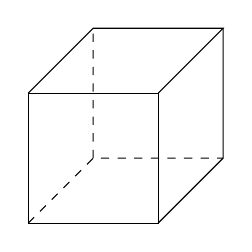
\begin{tikzpicture}[scale=0.55]
		%sichtbare Mantellinien
		\draw (0,0) -- (3,0) -- (3,3) -- (0,3) -- cycle;
		\draw (0,3) -- (1.5,4.5) -- (4.5,4.5) -- (3,3);
		\draw (4.5,4.5) -- (4.5,1.5) -- (3,0);
		%nicht sichtbare Mantellinien
		\draw[dashed] (0,0) -- (1.5,1.5) -- (4.5,1.5) (1.5,1.5) -- (1.5,4.5);
	\end{tikzpicture}
	&
	% Zylinder
	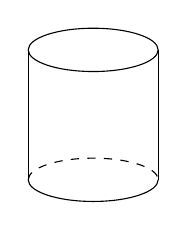
\begin{tikzpicture}[scale=0.55]
		%sichtbarer Teil der unteren Grundflaeche (vorderer Halbkreis)
		\draw (0,0.5) arc(-180:0:1.5cm and 0.5cm);
		%nicht sichtbarer Teil der unteren Grundflaeche (hinterer Halbkreis)
		\draw[dashed] (0,0.5) arc(180:0:1.5cm and 0.5cm);
		%linke Mantellinie
		\draw(0,0.5) -- (0,3.5);
		%obere Grundflaeche (vollstaendig sichtbar)
		\draw (0,3.5) arc(180:-180:1.5cm and 0.5cm);
		%rechte Mantellinie
		\draw (3,0.5) -- (3,3.5);
	\end{tikzpicture}
	&
	% Quader
	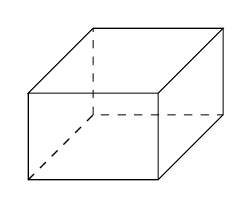
\begin{tikzpicture}[scale=0.55]
		%sichtbare Mantellinien
		\draw (0,2) -- (0,0) -- (3,0) -- (3,2) -- (0,2) -- (1.5,3.5) -- (4.5,3.5) -- (3,2);
		\draw (4.5,3.5) -- (4.5,1.5) -- (3,0);
		%nicht sichtbare Mantellinien
		\draw[dashed] (0,0) -- (1.5,1.5) -- (4.5,1.5) (1.5,1.5) -- (1.5,3.5);
	\end{tikzpicture}
	&
	% Dreiseitiges Prisma
	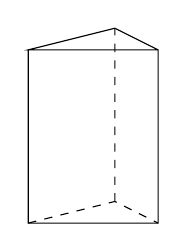
\begin{tikzpicture}[scale=0.55]
		%sichtbare Mantellinien
		\draw (0,4) -- (0,0) -- (3,0) -- (3,4) -- (0,4) -- (2,4.5) -- (3,4);
		%nicht sichtbare Mantellinien (hintere dreieckige Grundflaeche)
		\draw[dashed] (0,0) -- (2,0.5) -- (3,0) (2,0.5) -- (2,4.5);
	\end{tikzpicture}
	&
	% Kegel
	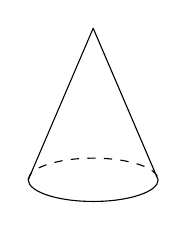
\begin{tikzpicture}[scale=0.55]
		%sichtbarer Teil der Grundflaeche (vorderer Halbkreis)
		\draw (0,0.5) arc(-180:0:1.5cm and 0.5cm);
		%nicht sichtbarer Teil der Grundflaeche (hinterer Halbkreis)
		\draw[dashed] (0,0.5) arc(180:0:1.5cm and 0.5cm);
		%linke Mantellinie
		\draw(0,0.5) -- (1.5,4);
		%rechte Mantellinie
		\draw (3,0.5) -- (1.5,4);
	\end{tikzpicture}
\end{mcquestionh}
\end{lstlisting}

\begin{ausgabe}
	\begin{mcquestionh}{Kreuzen Sie ALLE Körper an, die KEINE Prismen sind:}
		  % Wuerfel
		  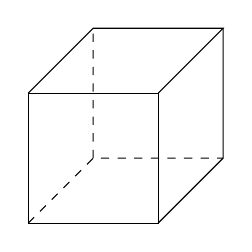
\begin{tikzpicture}[scale=0.55]
			    %sichtbare Mantellinien
			    \draw (0,0) -- (3,0) -- (3,3) -- (0,3) -- cycle;
			    \draw (0,3) -- (1.5,4.5) -- (4.5,4.5) -- (3,3);
			    \draw (4.5,4.5) -- (4.5,1.5) -- (3,0);
			    %nicht sichtbare Mantellinien
			    \draw[dashed] (0,0) -- (1.5,1.5) -- (4.5,1.5) (1.5,1.5) -- (1.5,4.5);
		  \end{tikzpicture}
		  &
		  % Zylinder
		  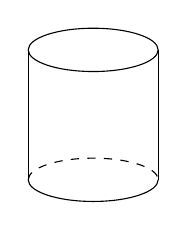
\begin{tikzpicture}[scale=0.55]
			    %sichtbarer Teil der unteren Grundflaeche (vorderer Halbkreis)
			    \draw (0,0.5) arc(-180:0:1.5cm and 0.5cm);
			    %nicht sichtbarer Teil der unteren Grundflaeche (hinterer Halbkreis)
			    \draw[dashed] (0,0.5) arc(180:0:1.5cm and 0.5cm);
			    %linke Mantellinie
			    \draw(0,0.5) -- (0,3.5);
			    %obere Grundflaeche (vollstaendig sichtbar)
			    \draw (0,3.5) arc(180:-180:1.5cm and 0.5cm);
			    %rechte Mantellinie
			    \draw (3,0.5) -- (3,3.5);
		  \end{tikzpicture}
		  &
		  % Quader
		  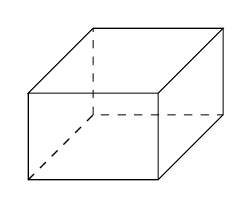
\begin{tikzpicture}[scale=0.55]
			    %sichtbare Mantellinien
			    \draw (0,2) -- (0,0) -- (3,0) -- (3,2) -- (0,2) -- (1.5,3.5) -- (4.5,3.5) -- (3,2);
			    \draw (4.5,3.5) -- (4.5,1.5) -- (3,0);
			    %nicht sichtbare Mantellinien
			    \draw[dashed] (0,0) -- (1.5,1.5) -- (4.5,1.5) (1.5,1.5) -- (1.5,3.5);
		  \end{tikzpicture}
		  &
		  % Dreiseitiges Prisma
		  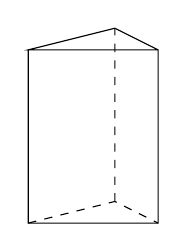
\begin{tikzpicture}[scale=0.55]
			    %sichtbare Mantellinien
			    \draw (0,4) -- (0,0) -- (3,0) -- (3,4) -- (0,4) -- (2,4.5) -- (3,4);
			    %nicht sichtbare Mantellinien (hintere dreieckige Grundflaeche)
			    \draw[dashed] (0,0) -- (2,0.5) -- (3,0) (2,0.5) -- (2,4.5);
		  \end{tikzpicture}
		  &
		  % Kegel
		  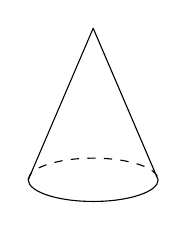
\begin{tikzpicture}[scale=0.55]
			    %sichtbarer Teil der Grundflaeche (vorderer Halbkreis)
			    \draw (0,0.5) arc(-180:0:1.5cm and 0.5cm);
			    %nicht sichtbarer Teil der Grundflaeche (hinterer Halbkreis)
			    \draw[dashed] (0,0.5) arc(180:0:1.5cm and 0.5cm);
			    %linke Mantellinie
			    \draw(0,0.5) -- (1.5,4);
			    %rechte Mantellinie
			    \draw (3,0.5) -- (1.5,4);
		  \end{tikzpicture}
	\end{mcquestionh}
\end{ausgabe}


%%%%  KAPITEL 5  %%%%
\section{Zusammenfassung}

Bei der Erstellung von Multiple-Choice-Fragen mit \hologo{LaTeX} lohnt es sich, einige bewährte Praktiken zu berücksichtigen. Achten Sie auf eine konsistente Formatierung, indem Sie für ähnliche Fragetypen stets die gleiche Umgebung verwenden. Dies erhöht nicht nur die Übersichtlichkeit für die Schülerinnen und Schüler, sondern erleichtert auch Ihnen als Lehrkraft die Erstellung und Wartung der Dokumente.

Die Wahl zwischen horizontalen und vertikalen MC-Fragen sollte sich nach der Länge der Antwortmöglichkeiten richten. Während sich horizontale Anordnungen ideal für kurze, prägnante Antworten eignen, bieten vertikale Formate mehr Platz für ausführlichere Optionen. Bei komplexen mathematischen Formeln in horizontalen MC-Fragen kann die Verwendung von \texttt{\textbackslash footnotesize} oder \texttt{\textbackslash small} die Lesbarkeit erheblich verbessern, indem sie die Formeln kompakter darstellen.

Eine gute Dokumentation Ihrer selbstdefinierten Befehle und Umgebungen zahlt sich langfristig aus. Kommentieren Sie daher Ihre Anpassungen sorgfältig. Für maximale Wiederverwendbarkeit empfiehlt es sich, die MC-Definitionen in eine separate \texttt{.tex}-Datei auszulagern, die Sie dann in verschiedenen Dokumenten per \texttt{\textbackslash input} einbinden können.

Die in dieser Handreichung vorgestellten Techniken demonstrieren, wie selbstdefinierte Befehle und Umgebungen die Erstellung von Multiple-Choice-Fragen in \hologo{LaTeX} erheblich vereinfachen. Mit \texttt{\textbackslash newcommand} und \texttt{\textbackslash newenvironment} können Sie eigene, auf Ihre Bedürfnisse zugeschnittene Strukturen definieren. Die horizontalen und vertikalen MC-Frage-Umgebungen bieten flexible Grundgerüste, die sich durch Farben, unterschiedliche Antwortanzahlen oder spezielle Formatierungen vielfältig anpassen lassen. Besonders interessant ist die Möglichkeit, Ti\textit{k}Z-Elemente als grafische Antwortoptionen zu verwenden, was besonders im MINT-Bereich neue didaktische Möglichkeiten eröffnet.

Mit diesem Werkzeugkasten lassen sich professionell gestaltete Multiple-Choice-Fragen für verschiedene Fachbereiche und Prüfungsformate erstellen. Die vorgestellten Grundstrukturen sind bewusst einfach gehalten, können aber leicht an eigene Bedürfnisse und Anforderungen angepasst werden – ganz im Sinne der Flexibilität und Anpassungsfähigkeit, die \hologo{LaTeX} auszeichnet.

\end{document}